\documentclass{standalone}
\usepackage[dvipsnames]{xcolor}
\usepackage{tikz}
\usetikzlibrary{arrows.meta}
\usetikzlibrary{positioning}

\colorlet{nphard}{Melon!50}
\colorlet{np}{SkyBlue!50}
\colorlet{p}{LimeGreen!50}

\begin{document}
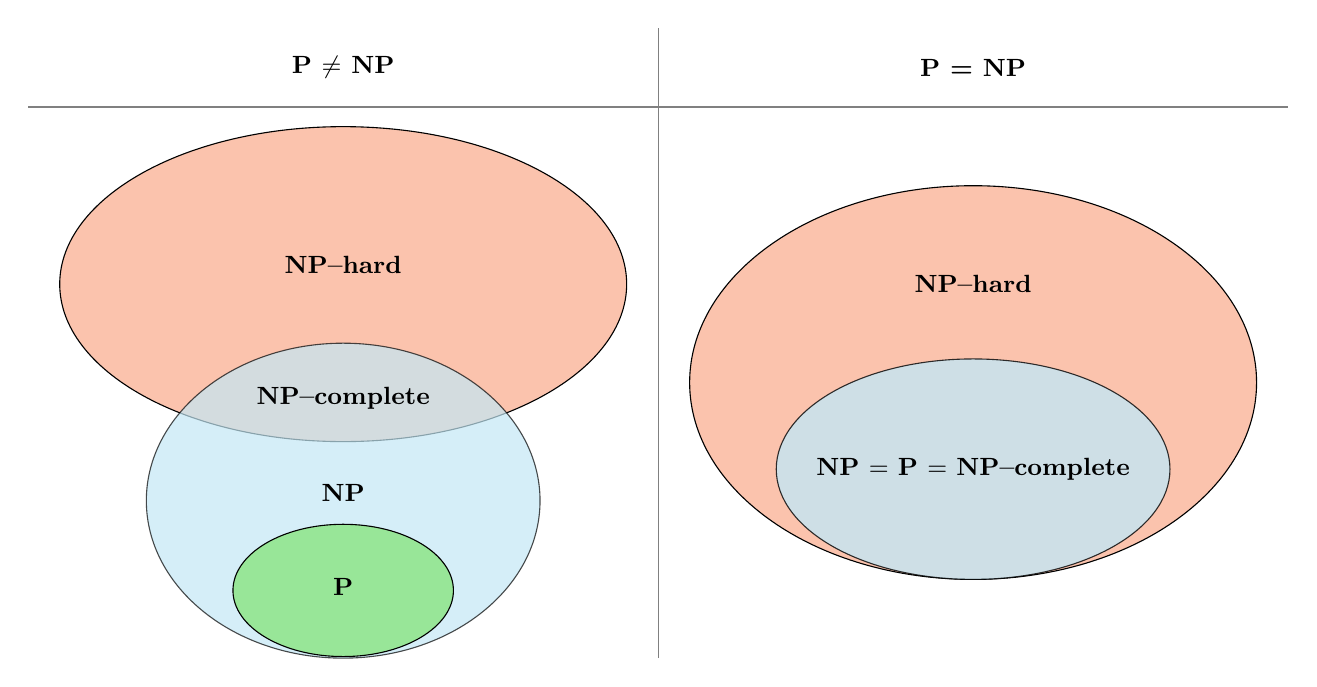
\begin{tikzpicture}

  % ---------- Left side (P != NP) ----------

  % Shapes
  \draw[fill=nphard] (0, 2.75) ellipse (3.6cm and 2.0cm);
  \draw[fill=np,opacity=0.7] (0, 0) ellipse (2.5cm and 2.0cm);
  \draw[fill=p] (0,-1.14cm) ellipse (1.4cm and 0.84cm);
  
  % Labels
  \node at (0, 0.1) (NP1) {\small\textbf{NP}};
  \node at (0, -1.1) (P1) {\small\textbf{P}};
  \node at (0, 1.3) (NPC1) {\small\textbf{NP--complete}};
  \node at (0, 3) (NPH1) {\small\textbf{NP--hard}};




  % ---------- Right side (P = NP)----------

  % Shapes
  \draw[fill=nphard] (8, 1.5) ellipse (3.6cm and 2.5cm);
  \draw[fill=np,opacity=0.8] (8, 0.4) ellipse (2.5cm and 1.4cm);
  

  % Labels
  \node at (8, 2.75) (NPH1) {\small\textbf{NP--hard}};
  \node[text width=4cm, align=center] at (8, 0.4) (PNP) {{\small\textbf{NP} = \textbf{P} = \textbf{NP--complete}}};


  % ---------- Titles ----------
  \node at (0, 5.5) (P1) {\small\textbf{P $\ne$ NP}};
  \node at (8, 5.5) (P1) {\small\textbf{P = NP}};

  % ---------- Lines ----------
  \draw[gray] (4, -2) -- (4, 6);
  \draw[gray] (-4, 5) -- (12, 5);
\end{tikzpicture}
\end{document}
